\chapter{Introduction}\label{chap:introduction}
\section{Galaxy}
Galaxy{\footnote{\url{https://usegalaxy.eu/}}} is an open-source biological data processing and research platform. It supports numerous types of extensively used biological data formats like FASTA, FASTAQ, GFF, PDB and many more. To process these datasets, it offers tools and workflows which transform these datasets (figure 1). Each tool and workflow furnish exclusive means to process datasets. A simple example of this processing is to merge two compatible datasets to make one. Another example can be to reverse complement a sequence of 
nucleotides\footnote{\url{https://usegalaxy.eu/?tool_id=MAF_Reverse_Complement_1&version=1.0.1&__identifer=zmk9dx9ivbk}}.

\begin{figure}[h]
\begin{centering}
    {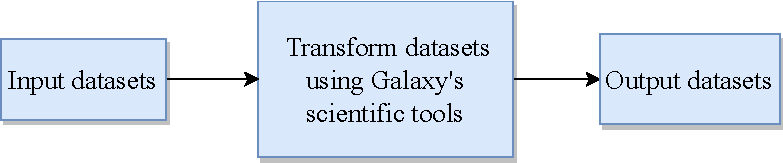
\includegraphics[scale=0.8]{figures/image_Galaxy_1.pdf}}
    \caption[Basic flow of dataset transformation]{\textbf{Dataset transformation}: The image shows a general flow of data transformation using Galaxy tools and workflows.}
\end{centering}
\end{figure}

A tool is a data-transforming entity. The tools are classified into multiple categories based on their functions and types. For example, the tools which manipulate text like replacing texts and selecting first lines of a dataset are grouped together under "Text Manipulation" category. These tools form the building blocks of workflows. The workflows are data processing pipelines where a set of tools are joined one after another and protrude from a tool to make branches. The connected tools should to be compatible with each other. It means that the output file types of one tool should be present in the input file types of the next tool.

\section{Galaxy tools}
A tool entails a specific function. It consumes a dataset, brings about some transformation and produces an output dataset which can be fed to other tools. It has multiple attributes which include its input and output file types, name, description, help text and so on. These attributes carry more information about a tool. When we look at the collective information about all these attributes for a set of tools, we recognize that some of them have comparable functionalities. There are tools which share affinities in their respective functions and the input and output file types they are glued to. For example, a tool "hicexplorer hicpca" \footnote{\url{https://usegalaxy.eu/?tool_id=toolshed.g2.bx.psu.edu/repos/bgruening/hicexplorer_hicpca/hicexplorer_hicpca/2.1.0&version=2.1.0&__identifer=5kcqmvb71gx}} has an output type named "bigwig". If there is a tool which also has "bigwig" as its input and/or output type, we consider there can be some similarity between these tools as they do transformations on similar types of files. In addition, we can find similar functions of tools by analyzing their "name" and "description" attributes. Let's take an example of two tools (figure 2):
 
\begin{figure}[h]
\begin{centering}
    {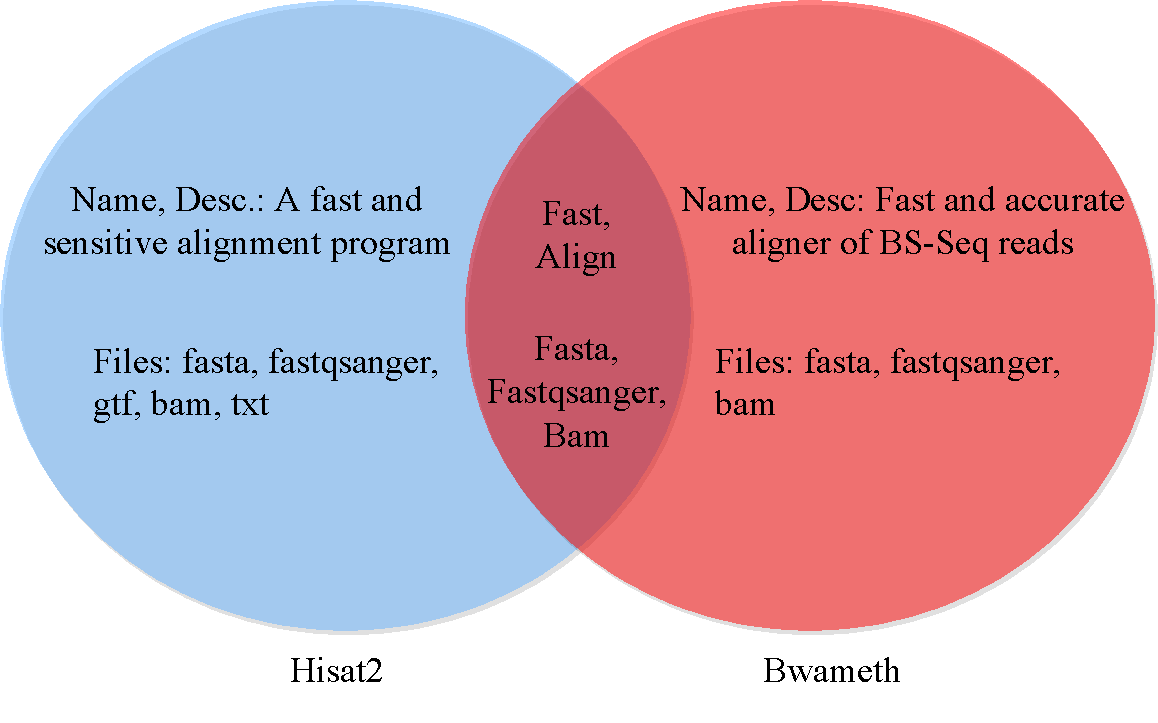
\includegraphics[scale=0.5]{figures/Venn_common_tools_info.pdf}}
    \caption[Common features of two tools using venn diagram]{\textbf{Common features of two tools using venn diagram}: The venn diagram shows the common features of two tools - linear regression and logistic regression. Based on these common features, we assess the extent of similarity between them.}
\end{centering}
\end{figure}

In figure 2, we take two tools - "linear regression" and "logistic regression" and collect their respective information from their input and output file types, name and description attributes. We can see that these tools share some features. They share a similar function of doing regression and few file types are also common. Similarly, if we extrapolate this notion of finding similar features among all the tools, we hope to find a set of similar tools for each tool. Also, it is possible that we end up with an empty set of similar tools for a tool.

\section{Motivation}
In figure 2, we see that there are tools which share characteristics. The Galaxy has thousands of tools having a diverse set of functions. Moreover, new tools keep getting added to the older set of tools. From a user's perspective, it is hard to keep knowledge about so many tools. In addition, it is important to make users aware of the presence of newly added tools if they are similar to some existing tool. If we can create a model which dispenses clues about a set of similar tools for each tool, it would give more options to users for their data processing using Galaxy. 

\begin{figure}[h]
\begin{centering}
    {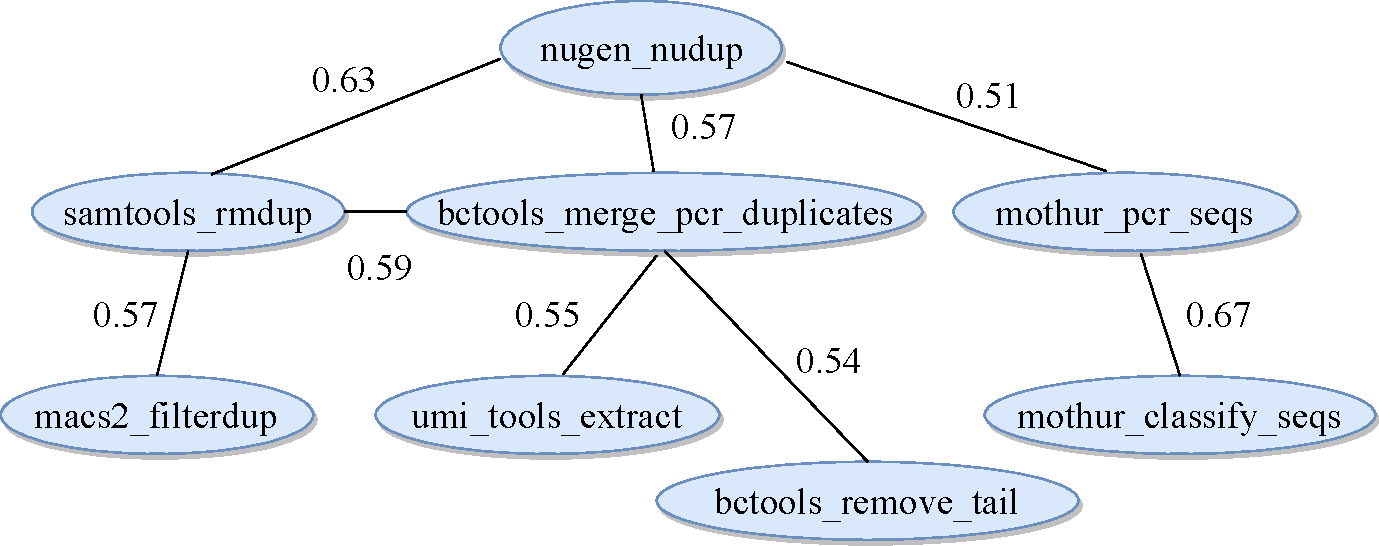
\includegraphics[scale=0.6]{figures/tools_sim_know_graph.pdf}}
    \caption[Similarity knowledge graph consisting of tools as nodes]{\textbf{Similarity knowledge graph consisting of tools as nodes}: The graph defines a network exhibiting relationship among the tools using similarity scores between a pair of tools (nodes). The similarity score shows the strength of similarity between a pair of tools.}
\end{centering}
\end{figure}

To elaborate it more, let's take an example of a tool "nugen nudup" \footnote{\url{ https://toolshed.g2.bx.psu.edu/repository?repository_id=4f614394b93677e3 }} (figure 3). It is used to find and remove PCR duplicates. The similar tools for it can be "samtools rmdup" and "bctools merge pcr duplicates" which also work on related concepts. These similar tools have their respective sets of similar tools and thereby make a network of related tools. This knowledge network exhibits "connectedness" among tools and can help users find multiple ways to process their data. The strength of this relation may vary from being small to large and we learn a continuous representation of the relation strength between a pair of tools and not a binary representation (which learns similar tool as 1 and dissimilar one as 0). Figure 3 shows how this similarity knowledge graph can evolve. First, we find similar tools for "nugen nudup" and connect them to their source tool specifying the similarity values as real numbers at the edges. These similar tools further have their own sets of similar tools and so on.